\section{Introduction}

\subsection{Objectives}

Blender is a complete 3D sofware, and can create 3D scenes from
scratch, from modeling to animation and render. The goal of this
project is to improve the open-source 3D software Blender, by
providing two new plug-ins to help artists creating rich environments.

Our aim is to add to Blender the possibility to generate large,
crowded environments. There are two independents parts: first
generate environments in a semi-automated way. Secondly, generate and
animate people in the environment. People's movements must be consistent
with the environment and other people's movements. There are some
examples of what has been created by some researchers in figures
\ref{fig:crowd} and \ref{fig:env}.

\begin{figure}[h] \centering

  \begin{subfigure}[t]{0.5\textwidth}
    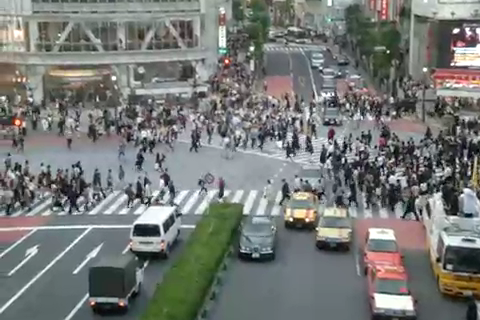
\includegraphics[width=7.5cm]{img/PLE_real.png}
    \caption{Real picture}
  \end{subfigure}% ~
  \begin{subfigure}[t]{0.5\textwidth}
    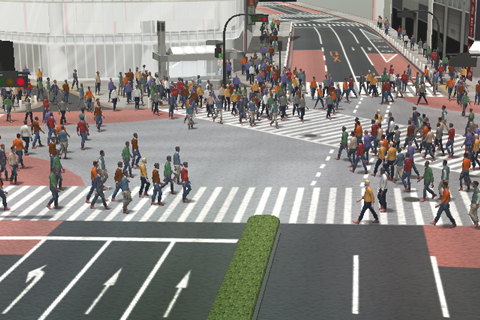
\includegraphics[width=7.5cm]{img/PLE_simu.png}
    \caption{Animation example from \cite{PLE}}
  \end{subfigure}
  \caption{A crossing in Tokyo}
  \label{fig:crowd}
\end{figure}

Note that Blend'it does not aim to be a realistic crowd generator, in
the sense of a usable simulator for sociological or scientific
experiments. The goal is to provide a complete generator for crowd and
environment for an artistic purpose only, that \textit{looks like} a
realistic crowd.

\begin{figure}[h]
  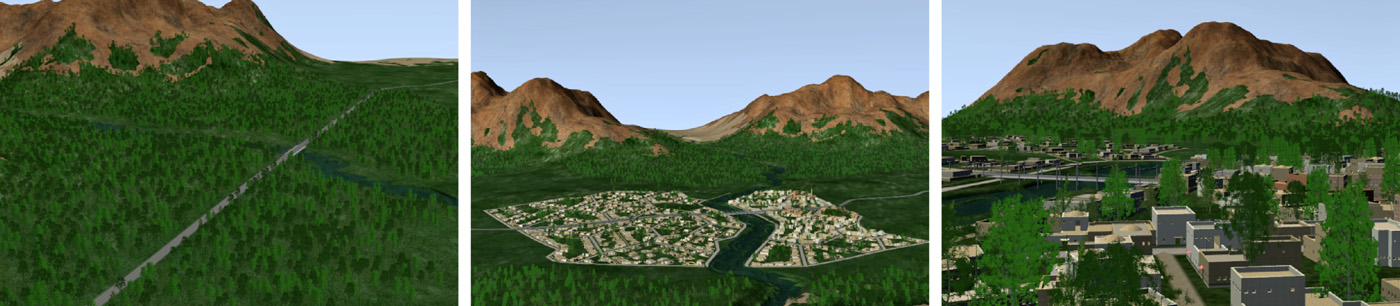
\includegraphics[width=15cm]{img/env1.jpg}
  \caption{Image taken from \cite{DeclarativeArchitecture}}
  \label{fig:env}
\end{figure}


There have been a lot of researches around the procedural generation
of crowds and environments in computer graphics. But the large
majority are implemented as research prototypes or in commercial
software. To the best of our knowledge, nothing exists for widely used
free software like Blender. 3D graphics is a domain that is still
closed-source, and every professional 3D artist uses costly
software. We think it is an important point to move some proprietary
technologies to the open-source world, to fill a little bit the gap.

\subsection{State of the art}

%% Reprendre remarque de l'expert : je crois que Massive est pas issu d'ilm ou un truc du genre
%% Reprendre des images du beamer ?


Animation of large crowds is really developed in the computer
graphics industry, enabling commercial 3D software to easily render
massive scenes with large crowds. For example, a software called Massive (\cite{Massive}) dramatically
changed the habits of 3D studios: it helped generating
the armies being displayed in \textit{Lord of the Rings}. The Golaem
(\cite{Golaem}) software is also able to render massive crowds in
different situations, and is used by the studio producing \textit{Game
of Thrones}. Nowadays, even commercial standalone 3D software like 3DS
MAX\cite{3dsmax} is able to generate realistic crowds. On the
contrary, no open-source software provides this kind of feature. In
the past, scripts had been developed, but they were not providing
realistic results, and are not working anymore.


\subsection{Team}

We are 9 Master students from the \textit{École Normale Supérieure de
Lyon}, France. As a part of our First year of Master in Research in
Computer Science, we need to develop and code a project of our choice
(here, ``Blend'it''), during the whole year. We are supervised by an
Associate Professor from the ENS Lyon, Eddy Caron. There is a project
leader, \me, and a deputy leader, \mr. Please do not hesitate to
contact us, by writing an email at \\
\textit{first name . last name@ens-lyon.fr}.\\

All our work is hosted on Github, and can be consulted on
\url{github.com/blendit}. We also have a website:
\url{blendit.github.io/}.


\subsection{Choice of Blender.}

The big advantage of producing a code based on Blender is that we can
use its Python API, which is very powerful. With it, one can
manipulate every objects and part of the Blender interface without
re-compiling Blender or even modifying the source code. Thus, we can
concentrate only one the new parts of the project: our algorithms, we
do not need to code another render engine for example.  The other
advantage is the Blender community, which already exists, and on which
we can rely to have feedback on our project.


\subsection{Structure of the project}

The two plug-in are currently independent, one is able to simulate the
motion of crowds, and one is able to generated environments. In each
plug-in, we split our code into a ``pure'' part, independent of
Blender, and one interacting with the Python API of Blender. This has
two advantages: we can test the ``pure'' part easily (testing the
Blender plug-in automatically is more difficult), and we may code
interface with other softwares too.



\paragraph{Outline}

\begin{itemize}
  \item In section 2, we present the work of the blender exploration team, done by \mr, \me and \ps.
  \item Section 3 presents the work done by \dl, \vl,
\js and \ps \ on the crowd simulation.
 \item Section 4 presents the environment
plug-in, done by \bb, \gc, \mr and \me.
%% \item Section 5 concludes this report.
\end{itemize}

  
